\section{Experiments}
\label{sec:experiments}

\subsection{Experimental Setup}
\label{sec:setup}
\paragraph{Datasets.}
We train the audiovisual generator on 284,218 clips
(approximately 500 hours) selected from the Seamless
training and development splits. This selection differs
from the full resource reported in
\cref{sec:data-statistics}.
We evaluate audiovisual backchannel generation on
Seamless and ResponseNet, and visual listening reactions
on ViCo.

\paragraph{Implementation details.}
We use LTX-2.3-22B~\cite{ltx_pending} as the audiovisual
generator, Qwen2.5-Omni-3B~\cite{qwen25omni} as the reaction
planner, and Whisper-large-v3~\cite{whisper} for speaker
audio encoding. Videos are processed at $512\times512$
resolution and 25 FPS, and speaker audio is resampled to
16\,kHz for Whisper. The Qwen planner is separately
fine-tuned with LoRA rank 32 and scaling parameter 64.
For LTX, we apply LoRA with rank and scaling parameter 8
to its native attention and feed-forward layers, while
fully training the additional Whisper attention branches.

Generator training uses 31 NVIDIA H200 GPUs with one
clip per GPU, BF16 mixed precision, and gradient
checkpointing. We use AdamW with
$(\beta_1,\beta_2)=(0.9,0.999)$, $\epsilon=10^{-8}$,
and zero weight decay. Learning rates are $10^{-5}$
for LTX LoRA, $3\times10^{-5}$ for the connector,
Whisper conditioning branch, and feature decoders,
and $10^{-4}$ for the event heads. Training is configured
for 9,169 iterations with 50 warm-up steps.
The loss weights are specified in \cref{eq:total}.
At inference, we use 30 Euler sampling steps with
video and audio CFG scales of \pending.

% \cnnote{引用与配置待补}{上述结构及维度已按当前配置和实际复用源码核对。Gemma的正式模型版本、LTX与Bernini的正式书目信息仍需补齐；源码定位见配套方法核对文档。生成训练中的Qwen未做规划SFT。}
% \cnnote{采样设置待冻结}{中文稿当前共享推理函数采用30步采样，视频／音频CFG为3／7。它们是可在实验中统一调整的参数，不是方法贡献。最终检查点、规划器及采样协议须共同确定后填写。}
% \cnnote{版本待冻结}{当前生成训练使用base Qwen hidden；最新LTX6000／6500＋SFT2752评测由SFT模型预测描述并重新提取H，属于“训练base H、推理SFT H”的配置。若最终主表采用该版本，须说明规划SFT及条件切换，并在所有对照中统一；本轮不把SFT自动并入AV＋Whisper＋Feature＋Event的四项设计。最终检查点、规划器和预算仍需冻结，不同batch／步数的终点不能直接当作等预算。}

\paragraph{Baselines and benchmarks.}

\cnnote{待补充}{}
% \cnnote{完整AV候选}{优先安排本文A0／A1及Qwen2.5-Omni→OVI系统对照。后者需适配允许安静和短反馈，固定模型与prompt，不能使用真实caption、事件或listener音轨。OmniResponse、OmniPersona、SpeakerVid-5M目前尚未获得可执行原生成器，先保留文献比较，不复制原表分数到本文短pair表。}
% \cnnote{视觉与额外输入对照}{GLARE需重训并披露Tref及previous motion来源；DyStream将self audio置零，Avatar Forcing将self audio和user视觉置零。L2L、DualTalk等保留额外动作／音轨条件时单列表，纯动作结果只在同表示空间比较；未核验renderer前不纳入视频表。RLHG、DIM、ReactFace、ListenFormer、LFI为资源允许时的扩展，不全部列为必做。}
% \cnnote{共同协议}{统一片段范围、参考帧、分辨率／帧率、音量处理、采样预算和失败处理，不用GT挑best-of-N。OVI1.1单次上限10秒而本任务可达11.95秒，需选择全部方法的共同窗口或公开分段／拼接协议，不能只截短基线。}
% \cnnote{原论文数值}{原协议文献表与本地实测分开。BFM/L1、EMOCA／DECA距离和不同含义的FD不混排；各论文RealTalk划分不视为统一测试。官方权重迁移、本文重训、第三方重实现及引用分别标注；协议不一致不计算相对提升。FID/FVD使用统一特征汇总，不平均分片分数。}

% Metrics are defined once here; results below refer back to this protocol.
\subsection{Evaluation Protocol}
\label{sec:evaluation}

\paragraph{Clip-level event agreement.}
Valid listening reactions can occur at different times,
making strict alignment with a single reference overly
restrictive. We therefore compare event-category presence
over each clip, counting repeated occurrences only once.
We report macro-precision, macro-recall, and macro-F1
separately for visual and vocal categories with reference
positives, and report false-positive rates for the remaining
categories. These scores measure category agreement with
the observed response, complementing the assessment of
contextual appropriateness.

\paragraph{Audiovisual quality and behavior.}
Building on the OmniResponse evaluation
framework~\cite{omniresponse}, we measure video quality
using PSNR, SSIM, LPIPS, FID, and FVD.
Emo-Acc, Emo-Div, and $\Delta$Resp characterize expression
agreement, expression diversity, and listening-motion
differences, following AnyTalker~\cite{anytalker}.
Audio diagnostics measure activity-duration error,
missed vocal responses, excess vocal duration, and false
vocalization on silent clips. Where applicable, SyncNet's LSE-D and LSE-C
measure lip synchronization. Unsupported cases are
reported as N/A, together with valid evaluation coverage.

\paragraph{Human evaluation.}
Human evaluation targets contextual appropriateness,
naturalness and engagement, and audiovisual coordination
(\cref{sec:qualitative}). The assessment allows alternative
reasonable reactions and natural quiet listening.

\subsection{Quantitative Comparisons}
\label{sec:quantitative}
\paragraph{Audiovisual backchannel generation.}
% Paragraph role P05: 完整视听任务的比较范围
The full-task comparison concerns listener audio, visual reactions, and their coordination (\cref{tab:av}). It uses current speaker audio and a listener first frame as inputs and does not treat supplied listener audio as generated audio.
% \cnnote{比较所能支持的结论}{已知listener音轨的动画对照只评价驱动画面；独立OVI的共享预测文本对照评价生成器，Qwen→OVI端到端对照评价系统，两者均不替代三组件消融。不同训练来源的迁移结果不能解释为共同训练下的架构因果优势。}
% \cnnote{定量结果待写}{完成同协议比较后，先写主表支持的最重要发现，再说明对应的媒体质量、反馈类别和声音诊断证据；如指标有取舍，明确写出。当前不预设本文优于基线。}
\begin{table*}[t]
    \centering\small
    \setlength{\tabcolsep}{2pt}
    \renewcommand{\arraystretch}{1.1}
    \begin{tabularx}{\textwidth}{@{}Y*{16}{r}@{}}
    \toprule
    & \multicolumn{6}{c}{Visual quality}
    & \multicolumn{4}{c}{Feedback behavior}
    & \multicolumn{3}{c}{Visual events}
    & \multicolumn{3}{c}{Audio events} \\
    \cmidrule(lr){2-7}
    \cmidrule(lr){8-11}
    \cmidrule(lr){12-14}
    \cmidrule(lr){15-17}
    Method
    & \makecell{CPBD\\$\uparrow$}
    & \makecell{PSNR\\$\uparrow$}
    & \makecell{SSIM\\$\uparrow$}
    & \makecell{FID\\$\downarrow$}
    & \makecell{FVD\\$\downarrow$}
    & \makecell{LPIPS\\$\downarrow$}
    & \makecell{Emo-Acc\\$\uparrow$}
    & Emo-Div
    & \makecell{$\Delta$Resp\\$\downarrow$}
    & \makecell{MLLM\\RDR}
    & \makecell{P\\$\uparrow$}
    & \makecell{R\\$\uparrow$}
    & \makecell{mF1\\$\uparrow$}
    & \makecell{P\\$\uparrow$}
    & \makecell{R\\$\uparrow$}
    & \makecell{mF1\\$\uparrow$} \\
    \midrule
    L2L~\cite{learningtolisten}
    & \pending & \pending & \pending & \pending & \pending &
    \pending
    & \pending & \pending & \pending & \pending
    & \pending & \pending & \pending
    & \NA & \NA & \NA \\
  
    DIM~\cite{dim}
    & \pending & \pending & \pending & \pending & \pending &
    \pending
    & \pending & \pending & \pending & \pending
    & \pending & \pending & \pending
    & \NA & \NA & \NA \\
  
    ViCo~\cite{vico}
    & \pending & \pending & \pending & \pending & \pending &
    \pending
    & \pending & \pending & \pending & \pending
    & \pending & \pending & \pending
    & \NA & \NA & \NA \\
  
    ListenFormer~\cite{listenformer}
    & \pending & \pending & \pending & \pending & \pending &
    \pending
    & \pending & \pending & \pending & \pending
    & \pending & \pending & \pending
    & \NA & \NA & \NA \\
  
    DyStream~\cite{dystream}
    & \pending & \pending & \pending & \pending & \pending &
    \pending
    & \pending & \pending & \pending & \pending
    & \pending & \pending & \pending
    & \NA & \NA & \NA \\
  
    GLARE~\cite{glare}
    & \pending & \pending & \pending & \pending & \pending &
    \pending
    & \pending & \pending & \pending & \pending
    & \pending & \pending & \pending
    & \NA & \NA & \NA \\
  
    Avatar Forcing~\cite{avatarforcing}
    & \pending & \pending & \pending & \pending & \pending &
    \pending
    & \pending & \pending & \pending & \pending
    & \pending & \pending & \pending
    & \NA & \NA & \NA \\

    Qwen2.5-Omni + LTX~\cite{avatarforcing}
    & \pending & \pending & \pending & \pending & \pending &
    \pending
    & \pending & \pending & \pending & \pending
    & \pending & \pending & \pending
    & \NA & \NA & \NA \\
    \midrule
    Ours
    & \pending & \pending & \pending & \pending & \pending &
    \pending
    & \pending & \pending & \pending & \pending
    & \pending & \pending & \pending
    & \pending & \pending & \pending \\
    \bottomrule
    \end{tabularx}
    \caption{Generation quality and feedback behavior comparison
    on [seamless dataset]. MLLM-RDR denotes the MLLM-based reaction
    detection rate. Event P, R, and mF1 are macro-averaged
    using clip-level category presence. Audio-event metrics
    are N/A for methods without generated audio.}
    \label{tab:av}
    \end{table*}

\paragraph{Shared visual-listening capabilities.}
% Paragraph role P06: 视觉对照与额外输入边界
The visual comparison concerns capabilities shared with video-only listening methods (\cref{tab:visual}). Methods that require additional inputs or produce only motion are considered separately; their results do not establish performance on the full audiovisual task.
\begin{table*}[t]
    \centering\small
    \setlength{\tabcolsep}{3pt}
    \begin{tabularx}{\textwidth}{@{}Yrrrrrrrrrr@{}}
    \toprule
    & \multicolumn{4}{c}{Feedback behavior}
    & \multicolumn{3}{c}{Visual events}
    & \multicolumn{3}{c}{Audio events} \\
    \cmidrule(lr){2-5}
    \cmidrule(lr){6-8}
    \cmidrule(lr){9-11}
    Method
    & \makecell{Emo-Acc\\$\uparrow$}
    & Emo-Div
    & \makecell{$\Delta$Resp\\$\downarrow$}
    & \makecell{MLLM\\RDR}
    & P$\uparrow$
    & R$\uparrow$
    & mF1$\uparrow$
    & P$\uparrow$
    & R$\uparrow$
    & mF1$\uparrow$ \\
    \midrule
    L2L~\cite{learningtolisten}
    & \pending & \pending & \pending & \pending
    & \pending & \pending & \pending
    & \NA & \NA & \NA \\
    DIM~\cite{dim}
    & \pending & \pending & \pending & \pending
    & \pending & \pending & \pending
    & \NA & \NA & \NA \\
    ViCo (RLHG)~\cite{vico}
    & \pending & \pending & \pending & \pending
    & \pending & \pending & \pending
    & \NA & \NA & \NA \\
    ListenFormer~\cite{listenformer}
    & \pending & \pending & \pending & \pending
    & \pending & \pending & \pending
    & \NA & \NA & \NA \\
    DyStream~\cite{dystream}
    & \pending & \pending & \pending & \pending
    & \pending & \pending & \pending
    & \NA & \NA & \NA \\
    GLARE~\cite{glare}
    & \pending & \pending & \pending & \pending
    & \pending & \pending & \pending
    & \NA & \NA & \NA \\
    Avatar Forcing~\cite{avatarforcing}
    & \pending & \pending & \pending & \pending
    & \pending & \pending & \pending
    & \NA & \NA & \NA \\
    \midrule
    Ours
    & \pending & \pending & \pending & \pending
    & \pending & \pending & \pending
    & \pending & \pending & \pending \\
    \bottomrule
    \end{tabularx}
    \caption{待确定 Feedback behavior comparison on [vico dataset].
    MLLM-RDR denotes the MLLM-based reaction detection rate.
    Event precision, recall, and F1 are macro-averaged separately
    for visual and audio categories using clip-level presence,
    without requiring temporal overlap with reference events.
    Emo-Div measures expression diversity without a preferred
    direction.}
    \label{tab:visual}
    \end{table*}

\subsection{Qualitative Results and Human Evaluation}
\label{sec:qualitative}
\paragraph{Qualitative comparisons.}
% \cnnote{样例计划}{图F5先放可替换布局。后续按预先说明的规则选择合理安静倾听、动作与短声共同表达、遗漏或不适当失败三类。每例保留speaker原音频、listener首帧、一个真实参考、各方法帧序列及各自音轨；同一时刻展示不代表必须与GT同时反应。动作标签说明人工／自动来源。完整视频待插入，不能只看波形判断类别与音质。}
\begin{figure*}[t]
\centering
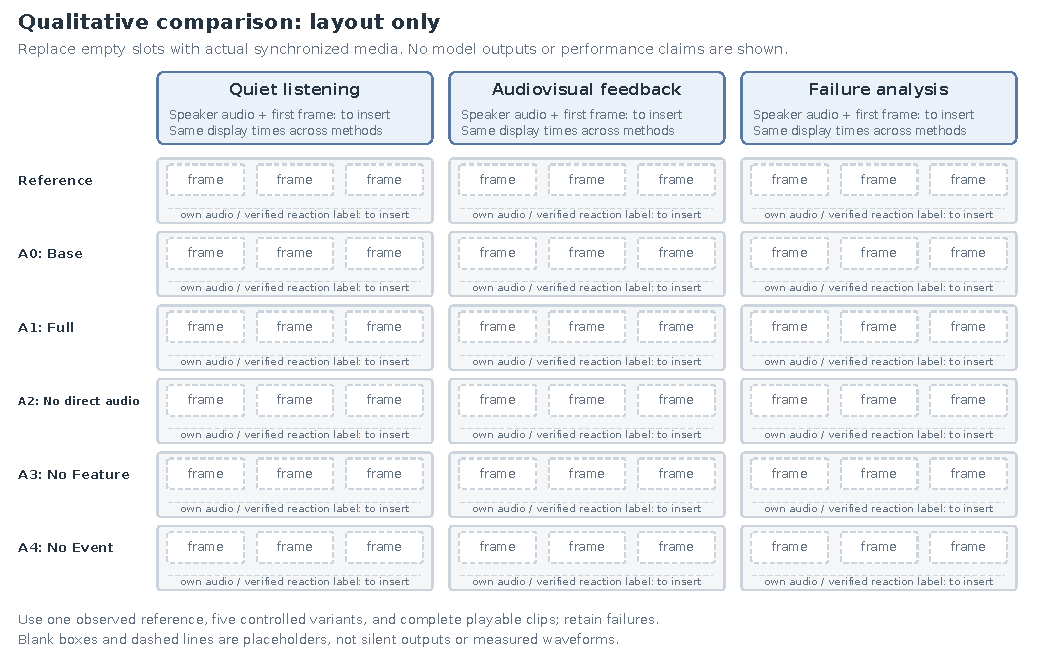
\includegraphics[width=\textwidth]{F5_results_layout.pdf}
\caption{\figdraft{F5: Qualitative comparison layout only} Three planned cases cover quiet listening, audiovisual feedback, and failure analysis. Rows reserve space for a reference response and the five ablation configurations. Every frame and audio slot is empty: this figure contains no generated result or claimed performance difference.}
\label{fig:qualitative}
\end{figure*}

\paragraph{Human evaluation.}
% \cnnote{人工评价计划}{在相同当前speaker音频与listener首帧条件下，匿名随机排序并由多位评分者判断适当性、参与感／自然度与声画协调（\cref{tab:human}）。画面／声音技术质量可分开评分。参考回应不是唯一正确答案，合理安静允许存在；无发声样本的相关协调项按协议记N/A并报告覆盖。人工仍需检查反应抢先、拖长或内部矛盾，不要求复现唯一GT时刻。}
% \cnnote{统计计划}{使用配对设计，按来源对话处理片段相关性，报告置信区间与有效样本。单次生成seed如实注明；样本bootstrap不替代训练多seed的不确定性。评分人数、量表／A-B形式及一致性统计待确定，不能预设自动指标与人评高度相关。}
 \begin{table*}[t]
    \centering\small
    \begin{tabularx}{\textwidth}{@{}Yccc@{}}
    \toprule
    Method
    & \makecell{Contextual\\appropriateness}
    & \makecell{Engagement /\\naturalness}
    & \makecell{Audiovisual\\coordination} \\
    \midrule
    Qwen+LTX
    & \pending & \pending & \pending \\
    GLARE
    & \pending & \pending & \NA \\
    DyStream
    & \pending & \pending & \NA \\
    Avatar Forcing
    & \pending & \pending & \NA \\
    Ours
    & \pending & \pending & \NA \\
    \bottomrule
    \end{tabularx}
    \caption{Human evaluation of contextual appropriateness,
    engagement and naturalness, and audiovisual coordination.
    Audiovisual coordination is not applicable to visual-only
    methods.}
    \label{tab:human}
    \end{table*}

\subsection{Ablation Studies}
\label{sec:ablation}

The full model combines the AV objective with Whisper
conditioning (W), clip-level event supervision (E),
and audiovisual feature supervision (F).
\Cref{tab:ablation} compares this model with three
variants: w/o W, w/o E, and w/o F. All configurations
retain the AV objective and Qwen/Gemma conditions.

These comparisons examine the contribution of direct
speaker-audio conditioning, event supervision for
feedback-category expression, and feature supervision
for adapting the conditioning representations to
listener audiovisual generation.

 \begin{table*}[t]
    \centering\small
    \begin{tabularx}{\textwidth}{@{}Ycccrrrrrr@{}}
    \toprule
    Configuration
    & W & F & E
    & FID$\downarrow$
    & FVD$\downarrow$
    & \makecell{Visual\\mF1$\uparrow$}
    & \makecell{Audio\\mF1$\uparrow$}
    & \makecell{Miss$\downarrow$\\(\%)}
    & \makecell{False$\downarrow$\\(\%)} \\
    \midrule
    Ours
    & \on & \on & \on
    & \pending & \pending & \pending
    & \pending & \pending & \pending \\
    \midrule
    w/o Whisper
    & \off & \on & \on
    & \pending & \pending & \pending
    & \pending & \pending & \pending \\
  
    w/o Feature
    & \on & \off & \on
    & \pending & \pending & \pending
    & \pending & \pending & \pending \\
  
    w/o Event
    & \on & \on & \off
    & \pending & \pending & \pending
    & \pending & \pending & \pending \\
    \bottomrule
    \end{tabularx}
    \caption{Component ablations.
    W denotes Whisper conditioning, F denotes audiovisual
    feature supervision, and E denotes clip-level event
    supervision on LTX hidden states. All configurations
    retain Qwen/Gemma conditioning and the AV objective.}
    \label{tab:ablation}
    \end{table*}
% \cnnote{受控条件与证据}{固定数据、标签、初始化、规划器、训练样本展示量和采样；可预生成同一预测描述供五组共用。训练仍用标注描述，测试用预测描述；GT描述对照另标oracle。W不能只用画质证明语义／韵律利用，F不能只用teacher重建损失证明最终媒体改善，E须同时看P/R/F1、误触发和合理安静倾听。}
% \cnnote{历史结果与扩展}{旧U-Event的6000／8000和新LTX6000＋SFT2752结果均不能代替这五组正式同条件结果。监督位置、整段／时序、两路Feature拆分和权重网格暂列可选；只有新增相应独立主张时再安排对照。}


\subsection{Data and Evaluation Validation}
\label{sec:validation}
\paragraph{Data and annotation quality.}
Validation protocols and quantitative checks remain \pending.
% \cnnote{资源与媒体抽检计划}{统计来源、角色、音轨、片段长度、人脸质量、有声／安静比例、逐类支持与共现。代表性随机抽检覆盖边界完整性、角色对应、音轨污染／过度截除和脸部可用性；稀有层过采样需按真实分布加权。资源分支关系放附录，正文保持最终规模简洁。}
% \cnnote{配对标注核验计划}{固定同批片段、Qwen3-Omni版本、采样设置与输出要求，比较仅音视频与加入带时间线索的匿名描述（\cref{tab:annotation}）。独立人工核验遗漏、无依据添加、顺序与发声内容；同时报告正确性和完整性。已有24条有声试点只能说明观察来源。若要声称数据处理提升生成效果，另需固定模型、规模和预算的训练对照。}
% \begin{table*}[t]
\centering\small
\caption{辅助标注质量表草案（待实施，可移至附录）。固定相同片段，对匿名描述进行独立人工核验；所有数值待填。}
\label{tab:annotation}
\begin{tabularx}{\textwidth}{@{}Yrrrrr@{}}
\toprule
标注设置 & 样本数 & 事件遗漏$\downarrow$ & 无依据添加$\downarrow$ & 顺序错误$\downarrow$ & 发声描述错误$\downarrow$ \\
\midrule
仅音视频 & \pending & \pending & \pending & \pending & \pending \\
音视频＋带时间反应线索 & \pending & \pending & \pending & \pending & \pending \\
\bottomrule
\end{tabularx}
\cnnote{统计口径待补}{各项分母、判定标准和分层抽样方式需先定义。检测线索不是人工真值；更长描述不直接表示更准确。媒体质量抽检另记录角色／切分合格率、音轨问题和脸部可用性。}
\end{table*}


% \paragraph{Event-evaluator reliability.}
% \cnnote{事件评测器核验}{在真实和生成媒体上分别抽样核验外部检测器，覆盖有声／无声、常见／稀有类及失败例；报告逐类质量、支持数和覆盖。训练弱负例不直接当测试负真值，未知／失败不当正确安静；不能用训练Event头自评。}
% \cnnote{本小节作用}{这里核验数据与测量工具是否可信；生成效果由主对比和消融回答，用户感受由前述人工评价回答。完成核验后报告具体发现，详细错误清单和逐类结果可放补充材料。}
% \cnnote{可选扩展与范围}{Whisper置零／错配、GT描述oracle、多seed、时长／发声／脸部质量分层和完整推理开销仅为可选诊断。错配可能产生条件冲突，不能单独证明理解；多样性需同时看适当性，不选best-of-N。推理开销包括描述、重编码、各编码器、生成与解码，不将片段吞吐叫流式延迟。本阶段不增加多轮历史、persona保持、全身或实时流式主张。}
% \cnnote{已有证据状态，按中文稿快照}{ViCo43已完成历史联合8000、DyStream和Avatar Forcing自动比较，人工评分为0；双200 LTX6000＋SFT2752有视频与活动结果，UTMOSv2无有效窗口，SyncNet／GLARE未运行；基础AV训练已启动，不能称五组完成。上述记录仅作筹备依据，当前不填正式结果表。}
